\documentclass[tikz,border=10pt]{standalone}
\usepackage{pgfplots}
\pgfplotsset{compat=1.18}

\begin{document}
	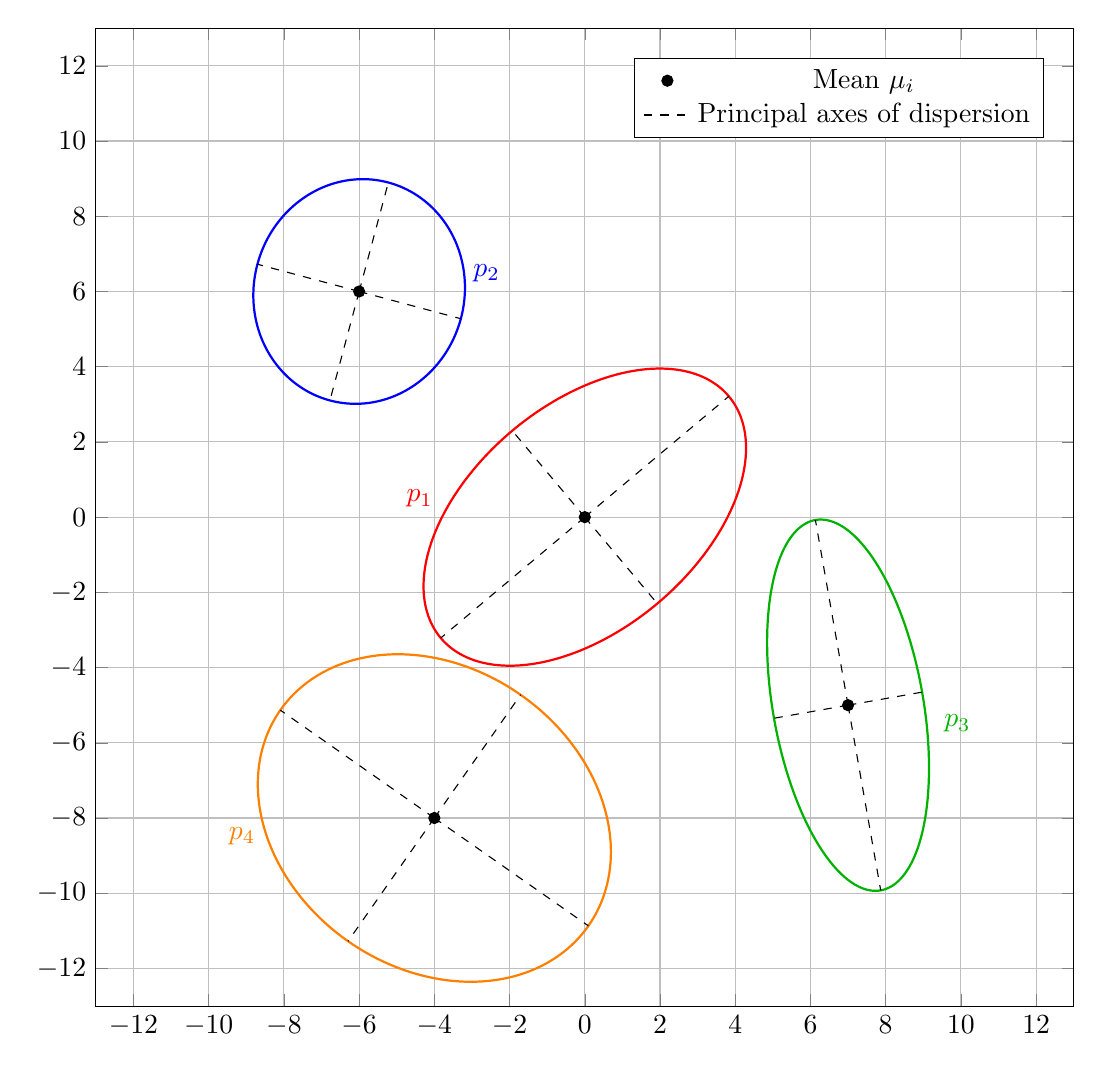
\begin{tikzpicture}
		\begin{axis}[
			grid,
			xmin=-13, xmax=13,
			ymin=-13, ymax=13,
			axis equal image,
			width=14cm,
			height=14cm,
			legend pos=north east,
			legend entries={Mean $\mu _i$, Principal axes of dispersion},
			]
			
			% Ellipse 1
			\addplot [
			domain=0:360, samples=100, smooth, thick, variable=\t, red,
			forget plot,
			]
			({0 + 5*cos(\t)*cos(40) - 3*sin(\t)*sin(40)}, 
			{0 + 5*cos(\t)*sin(40) + 3*sin(\t)*cos(40)});
			\addplot[only marks, mark=*, black, mark size=2pt, forget plot] coordinates {(0,0)};
			\draw[black, dashed] 
			(0,0) -- ({0 + 5*cos(40)},{0 + 5*sin(40)});
			\draw[black, dashed] 
			(0,0) -- ({0 - 5*cos(40)},{0 - 5*sin(40)});
			\draw[black, dashed] 
			(0,0) -- ({0 - 3*sin(40)},{0 + 3*cos(40)});
			\draw[black, dashed] 
			(0,0) -- ({0 + 3*sin(40)},{0 - 3*cos(40)});
			% Label ellipse 1
			\node[red, font=\bfseries] at (axis cs:-5,0) [anchor=south west] {$p_1$};
			
			% Ellipse 2
			\addplot [
			domain=0:360, samples=100, smooth, thick, variable=\t, blue,
			forget plot,
			]
			({-6 + 3*cos(\t)*cos(75) - 2.8*sin(\t)*sin(75)}, 
			{6 + 3*cos(\t)*sin(75) + 2.8*sin(\t)*cos(75)});
			\addplot[only marks, mark=*, black, mark size=2pt, forget plot] coordinates {(-6,6)};
			\draw[black, dashed] 
			(-6,6) -- ({-6 + 3*cos(75)},{6 + 3*sin(75)});
			\draw[black, dashed] 
			(-6,6) -- ({-6 - 3*cos(75)},{6 - 3*sin(75)});
			\draw[black, dashed] 
			(-6,6) -- ({-6 - 2.8*sin(75)},{6 + 2.8*cos(75)});
			\draw[black, dashed] 
			(-6,6) -- ({-6 + 2.8*sin(75)},{6 - 2.8*cos(75)});
			% Label ellipse 2
			\node[blue, font=\bfseries] at (axis cs:-2,6) [anchor=south east] {$p_2$};
			
			% Ellipse 3
			\addplot [
			domain=0:360, samples=100, smooth, thick, variable=\t, green!70!black,
			forget plot,
			]
			({7 + 2*cos(\t)*cos(10) - 5*sin(\t)*sin(10)}, 
			{-5 + 2*cos(\t)*sin(10) + 5*sin(\t)*cos(10)});
			\addplot[only marks, mark=*, black, mark size=2pt, forget plot] coordinates {(7,-5)};
			\draw[black, dashed] 
			(7,-5) -- ({7 + 2*cos(10)},{-5 + 2*sin(10)});
			\draw[black, dashed] 
			(7,-5) -- ({7 - 2*cos(10)},{-5 - 2*sin(10)});
			\draw[black, dashed] 
			(7,-5) -- ({7 - 5*sin(10)},{-5 + 5*cos(10)});
			\draw[black, dashed] 
			(7,-5) -- ({7 + 5*sin(10)},{-5 - 5*cos(10)});
			% Label ellipse 3
			\node[green!70!black, font=\bfseries] at (axis cs:9.3,-5) [anchor=north west] {$p_3$};
			
			% Ellipse 4
			\addplot [
			domain=0:360, samples=100, smooth, thick, variable=\t, orange,
			forget plot,
			]
			({-4 + 4*cos(\t)*cos(55) - 5*sin(\t)*sin(55)}, 
			{-8 + 4*cos(\t)*sin(55) + 5*sin(\t)*cos(55)});
			\addplot[only marks, mark=*, black, mark size=2pt, forget plot] coordinates {(-4,-8)};
			\draw[black, dashed] 
			(-4,-8) -- ({-4 + 4*cos(55)},{-8 + 4*sin(55)});
			\draw[black, dashed] 
			(-4,-8) -- ({-4 - 4*cos(55)},{-8 - 4*sin(55)});
			\draw[black, dashed] 
			(-4,-8) -- ({-4 - 5*sin(55)},{-8 + 5*cos(55)});
			\draw[black, dashed] 
			(-4,-8) -- ({-4 + 5*sin(55)},{-8 - 5*cos(55)});
			% Label ellipse 4
			\node[orange, font=\bfseries] at (axis cs:-8.5,-8) [anchor=north east] {$p_4$};
			
			% Point noir (Mean) pour la légende
			\addplot[only marks, mark=*, black, mark size=2pt] coordinates {(20,20)};
			
			% Segment noir tireté (Axes) pour la légende
			\addplot[black, dashed, thick, domain=0:1, samples=2, forget plot=false] ({20 + \x}, {20});
			
		\end{axis}
	\end{tikzpicture}
\end{document}
